\chapter{Introduction} \label{introducao}


Autonomous vehicles (AV) can significantly improve road safety and reduce accidents, as most accidents are caused due to human errors. The market penetration rate of AVs is estimated to be between 24\% and 87\% by 2045 \cite{bansal2017forecasting}. According to the German Statistical Department, the number of car crashes in Germany was over 2 million, just in 2019, and some levels of AV can support to reduce this amount \cite{deutsch}, and more than 90 percent of crashes are caused by human errors \cite{car-crash}. 


It is possible to create high impact applications in this area, establishing interrelations and information flows to detect new extended stimuli in scenarios where the infrastructure is physical or mobile \cite{bayat2017environmental}. There is also the possibility of applying computer vision (CV) concepts that allow the car to perceive the external environment. Combined with CV tools, the vehicle can interpret the external scenario and connect these outputs using Machine Learning (ML) approaches \cite{rasouli2019autonomous}.

One significant challenge for AV is to estimate the distance from the surrounding objects. It is possible to perform this task using the vehicle to infrastructure (V2I) communications or other techniques, such as Global Positioning System (GPS) \cite{hobert2015enhancements}. Therefore, some studies investigate the AV's acceptance to demonstrate that this new technology can reduce car accidents. A research guided by Xu et al. shows that, among the respondents, 42.35 \% and 45.28 \% expect low risk and lower insurance premiums for autonomous vehicles, respectively \cite{xu2019autonomous}.

Considering the possibility of using cameras around the road, this thesis proposes an object detection model using a multi-camera approach. We also implement algorithms responsible for detecting and classifying objects and estimating the distance of the object's position.

\section{Motivation}

Autonomous vehicles are an upcoming reality for future years. Following this trend, it is essential to develop new solutions. In particular, vehicle tracking has become a significant necessity. Wider AV adoption should reduce traffic jams and decrease the number of car crashes \cite{bonnefon2016social}. There are many self-drive car automation levels until full automation is reached, as shown in Figure \ref{fig:automation}. 

The proposal of this work deals with driving test scenarios of AVs. Monitoring test trials using drones is limited to drone's battery life, amounting to 30 to 45 minutes \cite{9138314}. This work uses infrastructure that can be positioned along the road as a pole-mounted camera that sends the data to a command center.

\begin{figure}[H]
\centering
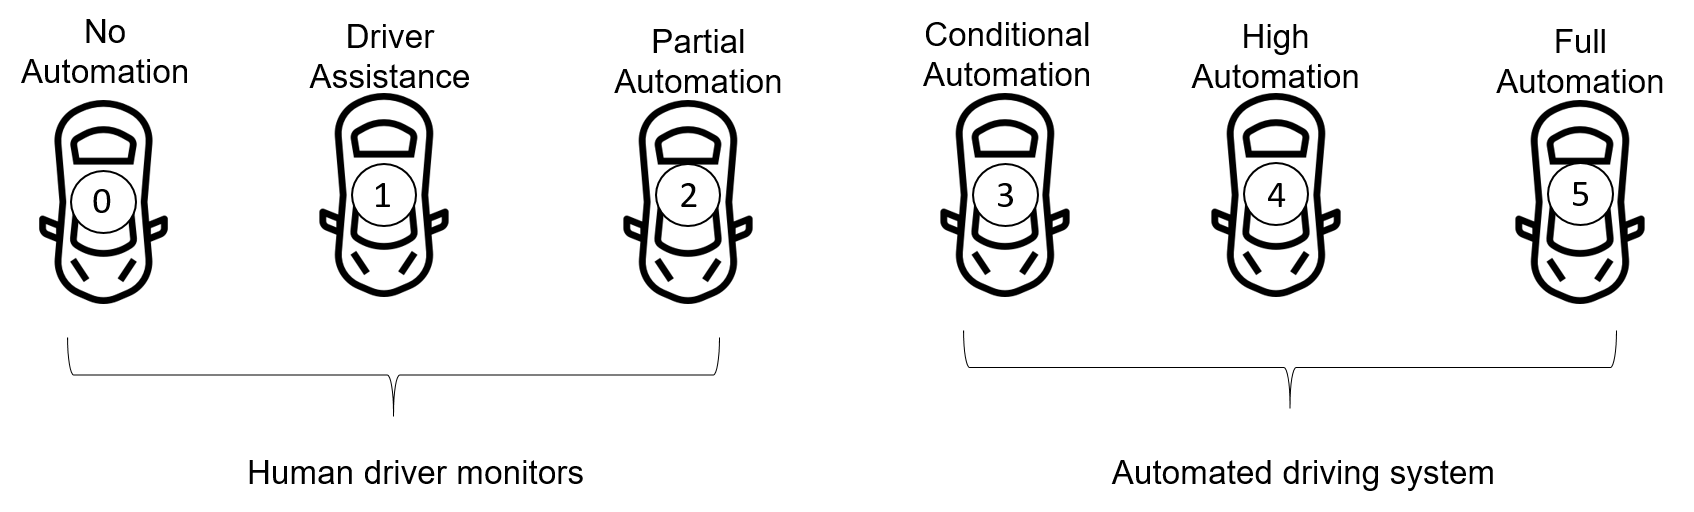
\includegraphics[scale=0.6]{imagens/Levels.png}
\caption{Levels of driving automation}
\label{fig:automation}
\end{figure}

\section{Problem Description}

It is to create an architecture to detect objects and to measure their distance along the road. A possible approach is using drones, but it is not ideal due to the battery life limitation for long tests, as illustrated in Figure \ref{fig:tests}. The goal is to track the position of the cars, namely vehicles under the test (VUT) and traffic simulation vehicles (TSV) along the test track, and send this information to the command central (CC). 

\begin{figure}[H]
\centering
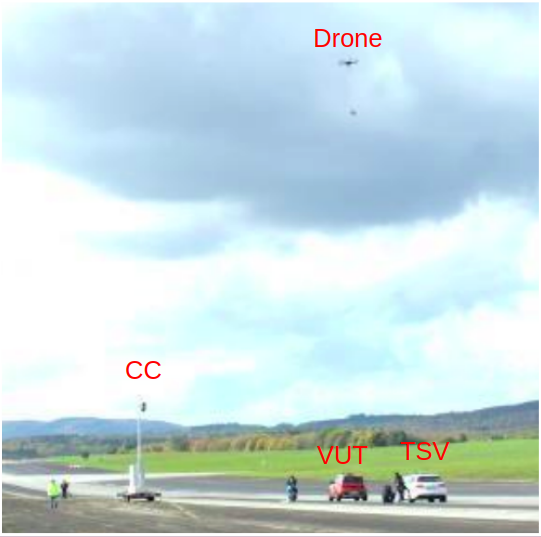
\includegraphics[scale=0.55]{imagens/proposal.png}
\caption{Modelling of the test track scenario using drones, CC designates the command central, VUT is the vehicle under test and TSV is a traffic simulation vehicle.}
\label{fig:tests}
\end{figure}

\section{Objectives}

The main objective is to create a framework to detect objects such as cars, trucks, motorcycles, pedestrians, and other arbitrary obstacles along the road. Additionally, the framework must also estimate the distance of such objects using a camera array.

\section{Published Works}

Simultaneously, with this work's development, the author has worked in several computer sciences domains, particularly in the data science domain, keeping the multidisciplinary mind. The following works were published along with the pursuit of the Master's Degree:

\begin{enumerate}

\item \textbf{PRACIANO, BRUNO J. G.}; DE CALDAS FILHO, FRANCISCO L. ; E MARTINS, LUCAS M. C. ; DA CUNHA, DAYANNE F. ; DA SILVA, DANIEL ALVES ; DE SOUSA JÚNIOR, RAFAEL TIMÓTEO. SEGURANÇA DO AMBIENTE USANDO DISPOSITIVO IOT COM PROCESSAMENTO DISTRIBUÍDO. In: Atas da conferência IberoAmericana WWW/Internet 2019, 2019. Atas da conferência Ibero-Americana WWW/Internet 2019, 2019. p. 163

\item MARQUES, Angelica Alves da Cunha; \textbf{PRACIANO, Bruno Justino Garcia}. Researchers of the Brazilian archivistics scientific community in French international areas of interlocution Encontros Bibli: revista eletrônica de biblioteconomia e ciência da informação, Florianópolis, v. 25, p. 01-14, mar. 2020. ISSN 1518-2924. doi:https://doi.org/10.5007/1518-2924.2020.e65864.

\item CASTELINO, R. M.; MOREIRA, G. P.; \textbf{PRACIANO, BRUNO JUSTINO GARCIA}; SANTOS, GIOVANNI A.; WEICHENBERGER, L.; DE SOUSA, JR, RAFAEL T. Improving the accuracy of pedestrian detection in partially occluded or obstructed scenarios. In: 2020 10th International Conference on Advanced Computer Information Technologies, 2020, Deggendorf. 2020 10th International Conference on Advanced Computer Information Technologies, 2020.

\item CANEDO, EDNA; PINHEIRO, GABRIEL; SOUSA JR., RAFAEL; RIBEIRO, RENATO; \textbf{PRACIANO, BRUNO}; LOPES DE MENDONÇA, FÁBIO. Front End Application Security: Proposal for a New Approach. In: 22nd International Conference on Enterprise Information Systems, 2020, Prague. Proceedings of the 22nd International Conference on Enterprise Information Systems, 2020. p. 233.

\item SOUSA JR., RAFAEL; LOPES DE MENDONÇA, FÁBIO; NZE, GEORGES; PINHEIRO, GABRIEL; \textbf{PRACIANO, BRUNO }; CANEDO, EDNA. Performance Evaluation of Software Defined Network Controllers. In: 10th International Conference on Cloud Computing and Services Science, 2020, Prague. Proceedings of the 10th International Conference on Cloud Computing and Services Science, 2020. p. 363.


\item SILVA, DANIEL ALVES DA; TORRES, JOSÉ ALBERTO SOUSA; PINHEIRO, ALEXANDRE; DE CALDAS FILHO, FRANCISCO L.; MENDONÇA, FABIO L. L.; \textbf{PRACIANO, BRUNO J. G}; KFOURI, GUILHERME OLIVEIRA; DE SOUSA, JR, RAFAEL T. Inference of driver behavior using correlated IoT data from the vehicle telemetry and the driver mobile phone. In: 2019 Federated Conference on Computer Science and Information Systems, 2019. org.crossref.xschema.\_1.Title@7d70270b, 2019. p. 487.

\item KFOURI, GUILHERME DE O. ; GONÇALVES, DANIEL G. V. ; DUTRA, BRUNO V. ; ALENCASTRO, JOÃO F. DE ; FILHO, FRANCISCO L. DE CALDAS ; MARTINS, LUCAS M. C. E ; \textbf{PRACIANO, BRUNO J. G.} ; ALBUQUERQUE, ROBSON DE O. ; JR, RAFAEL T. DE SOUSA . Design of a Distributed HIDS for IoT Backbone Components. In: 2019 Federated Conference on Computer Science and Information Systems, 2019. org.crossref.xschema.\_1.Title@7bad8b1f, 2019. p. 81.

\item DE MENDONCA, FABIO L. L.; DA CUNHA, DAYANNE F.; \textbf{PRACIANO, BRUNO J. G.}; DA ROSA ZANATTA, MATEUS; DA COSTA, JOAO PAULO C. L.; DE SOUSA, RAFAEL T. P2PIoT: A Peer-To-Peer Communication Model for the Internet of Things. In: 2019 Workshop on Communication Networks and Power Systems (WCNPS), 2019, Brasilia. 2019 Workshop on Communication Networks and Power Systems (WCNPS), 2019. p. 1.

\item BRANDAO, IURE V.; DA COSTA, JOAO PAULO C. L.; SANTOS, GIOVANNI A.; \textbf{PRACIANO, BRUNO J}. G.; JUNIOR, FRANCISCO C. M. D.; DE S. JUNIOR, RAFAEL T. Classification and predictive analysis of educational data to improve the quality of distance learning courses. In: 2019 Workshop on Communication Networks and Power Systems (WCNPS), 2019, Brasilia. 2019 Workshop on Communication Networks and Power Systems (WCNPS), 2019. p. 1.


\item DO NASCIMENTO SILVA, GERSON ; DE CALDAS FILHO, FRANCISCO LOPES ; DOS REIS, VINICIUS ELOY ; \textbf{PRACIANO, BRUNO JUSTINO }; LUSTOSA, JOÃO PAULO ; DE SOUSA JÚNIOR, RAFAEL TIMÓTEO . MODELO DE REDES NEURAIS ARTIFICIAIS EM SUPORTE TECNOLÓGICO À DETECÇÃO DE CARTEIS EM LICITAÇÕES PÚBLICAS. In: Atas da conferência IberoAmericana WWW/Internet 2019, 2019. Atas da conferência Ibero-Americana WWW/Internet 2019. p. 191.

\end{enumerate}

\section{Chapters Description}

This work is structured as follows: in Chapter 2, state of the art is presented to support this work, exploring previous contributions in this research area, the theoretical concepts necessary to the understanding of this work, and as self-driving cars are a new trend topic, it is essential to describe in greater detail.  Chapter 3 shows the proposed framework, and mathematical modeling is presented. Chapter 4 discusses the results achieved, algorithm performance, and the error for object detection and position estimation. Finally, in Chapter 5, the concluding remarks are made regarding the experiments and future works' suggestions.


